Es la representación visual de la magnitud de la STFT, y contrapone gráficamente tiempo y frecuencia haciendo un gradiente de color a más oscuro según se incrementa la más intensidad/magnitud presente la señal en ese punto.

Existen diferentes tipos, en función de cómo se traten los respectivos elementos de la STFT (magnitud, cuadrado, logarítmico, logarítmico cuadrado). Se puede observar cómo varía su generación en función del tratamiento de la STFT en la Figura \ref{fig:EspectrogramasSTFT} y que se diferencian en lo siguiente:

\begin{itemize}[
    itemsep=0.5em,
    topsep=0.5em,
    parsep=0pt,
    partopsep=0pt
]
    \item El espectrograma de magnitud muestra directamente la amplitud de cada frecuencia. Se diferencia del espectrograma de potencia en que la diferencia entre una componente débil de la señal y una fuerte es menor y de los dos gráficos inferiores porque al utilizar una escala lineal las componentes más fuertes dominan el color y las más débiles quedan oscuras.
    \item El espectrograma de potencia representa el cuadrado de la magnitud. Se diferencia del gráfico de magnitud porque en este los valores mayores que uno aumentan considerablemente y los pequeños se reducen todavía más, es decir, existe un rango mas amplio entre valores fuertes y débiles. 
    \item El espectrograma logarítmico aplica un logaritmo a la magnitud. Se diferencia de los espectrogramas de magnitud superiores en que al aplicarse un logaritmo se reduce el rango dinámico y con ello la diferencia visual entre componentes fuertes y débiles y por eso se muestra con más brillo y texturas. 
    \item El espectrograma logarítmico potencia aplica un logaritmo a la potencia de la magnitud. Se diferencia de los espectrogramas superiores en que se recuperan los valores que quedan ocultos en la escala lineal, y del logaritmo de magnitud en que al apartir de los valores elecados al cuadrado las regiones energéticas resaltan más y las débiles quedan mas ocultas.
\end{itemize}

\begin{figure}[H]
    \centering
    \makebox[\textwidth][c]{%
        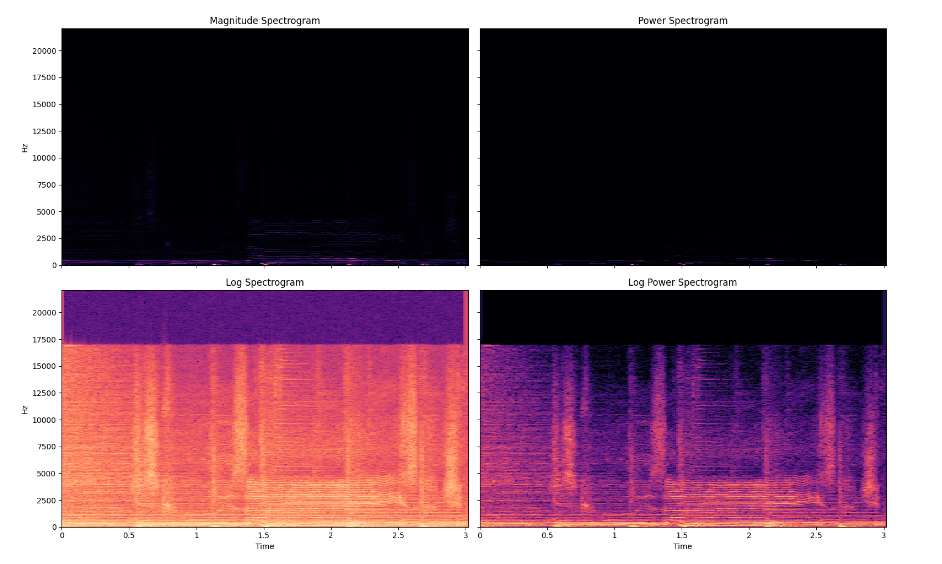
\includegraphics[
            width=1.25\textwidth,
            keepaspectratio
        ]{commons/Fig4.png}%
    }
    \caption{Diferentes generaciones de espectrogramas según el tratamiento de la STFT.}
    \label{fig:EspectrogramasSTFT}
\end{figure}

Por lo general en procesamiento de audio se utiliza un tipo especial: los espectrogramas de Mel. Un espectrograma de Mel es similar a un espectrograma común en el sentido de que muestra el contenido de frecuencia de una señal de audio a lo largo del tiempo pero en un eje de frecuencia diferente. En un espectrograma estándar, el eje de frecuencia es lineal y se mide en hercios (Hz), pero sin embargo el sistema auditivo humano es más sensible a los cambios en las frecuencias bajas que en las frecuencias altas, y esta sensibilidad disminuye de manera logarítmica a medida que la frecuencia aumenta. La escala mel es una escala perceptual que aproxima la respuesta de frecuencia no lineal del oído humano. \cite{HuggingFaceCourse}. En la Figura 4.6 se muestra la diferencia en la representación visual de ambos métodos. 

Si bien el espectrograma común que se utiliza en procesamiento de audio es el de Mel, en este trabajo se ha optado por mostrar el contenido de la frecuencia de una señal de audio utilizando espectrogramas estándar. La principal razón detrás de esta elección es porque el espectrograma Mel representa sonido de una manera más afin a la percepción humana, de manera que realmente se pierde información, mientras que el espectrograma STFT lineal conserva una correspondencia exacta entre frecuencia máscara magnitud y fase. Como el sistema desarrollado trabaja estimando máscaras a applicar sobre la magnitud STFT de la mezcla, la representación lineal es la opción natural: la máscara se estima en el mismo espacio donde se aplica y donde posteriorrmente se realiza la reconstrucción.


\begin{figure}[H]
    {\begin{center}
    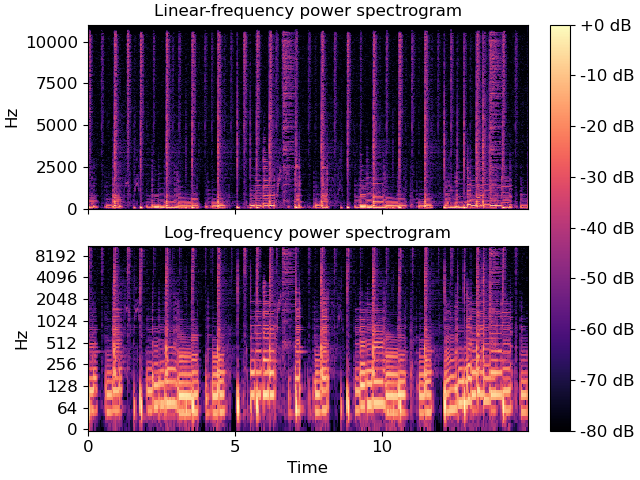
\includegraphics[width=0.7\textwidth]{commons/SpectrogramNormalMel.png}
    \caption{Espectrograma estándar arriba y espectrograma de Mel abajo.}
    \label{fig:EspectrogramasNormalMel}
    \end{center}}
\end{figure}
